Speech Foundation Models (SFMs) have become extremely popular in recent years.
These models are pretrained using either self-supervised learning~(SSL)~\cite{hsu2021hubert,Baevski_wav2vec2,Chen2021WavLMLS,baevski22_data2vec} or a supervised learning~(SL)~\cite{radford23_whisper} objective on large scale training data.
A major appeal of SFMs is that after initial large-scale training, they can be transferred to new downstream tasks with a relatively modest amount of new training data.
Prior literature has demonstrated the generalizability of SFM representations across various downstream speech processing tasks~\cite{yang_SfmEval,shi23g_mlsuperb}, including Automatic Speech Recognition (ASR)~\cite{baevski2021wav2vec-u,liu2022wav2vec-u2}, Speech Segmentation~\cite{peng2022vghubert,Strgar_2022}
Visually Grounded Speech~\cite{shihSpeechCLIP,layne_mspchclip}, Speaker Verification~\cite{aldeneh24_SVDS} and Emotion Recognition~\cite{Morais_emotion_ssl}.
% \david{maybe add citations for ER and LID}

%Speech Foundation Models (SFMs) have gained significant popularity in recent years. 
%These speech encoders are pretrained using either self-supervised~\cite{hsu2021hubert,Baevski_wav2vec2,Chen2021WavLMLS,baevski22_data2vec} or supervised objectives~\cite{radford23_whisper} on large-scale datasets. 
%SFMs gain its popularity in various speech-related application scenario by reducing the need for labeled training data.
%Prior studies have demonstrated their generalizability across multiple downstream speech processing tasks~\cite{yang_SfmEval,shi23g_mlsuperb}, including Automatic Speech Recognition (ASR)~\cite{baevski2021wav2vec-u,liu2022wav2vec-u2}, Speech Segmentation~\cite{peng2022vghubert,Strgar_2022}
%Visually Grounded Speech~\cite{shihSpeechCLIP,layne_mspchclip} and Speaker Verification~\cite{aldeneh24_SVDS}.


% talk about fusion
% \ian{talk about fusion from ensemble and bagging}
Despite their strong representations, researchers have explored methods to further enhance the effectiveness of SFMs.
One such approach involves fusing multiple speech encoders to obtain more powerful representations for downstream tasks. 
This concept dates back to the 1990s as ``ensemble learning''~\cite{Hansen90_ensemble,schapire90_strength,Breiman96_BaggingP,Freund_adaboost} whereby weak classifiers can be combined into a strong classifier.
Ensembling models can improve generalization ability by leveraging diverse training data distributions and model architectures.
Since SFMs are pretrained using different objectives and different data distributions (varying in acoustic conditions, speaker distributions, and content domains), it is reasonable to combine multiple SFMs to boost performance and robustness.
Several works have shown the benefits of SFM fusion in tasks such as ASR~\cite{tang22_fusion,fu23b_otf}, MOS Prediction~\cite{yang22o_mosFusion}, and Emotion Recognition~\cite{morais22_erFusion}.

% talk about layer selection
Another direction for improving SFMs is optimizing the approach of fusing information across speech encoder layers.
As observed in~\cite{Ankita2022CCA}, different layers of self-supervised speech models tend to encode different aspects of speech information in an input utterance. 
In general, lower layer representations are highly correlated with the acoustic waveform itself, while deeper layers encode more abstract representations such as phonetic identity.
% Because SSL models are used for many different downstream tasks,
To leverage SSL models on many different downstream tasks,
a commonly used approach (such as in the SUPERB~\cite{yang21c_superb} benchmark) is to compute a weighted sum over all layer representations (with trainable weights) from the upstream SSL model which is then used as the input to the downstream model. 
In doing so, the extracted information from the SSL model is not limited to a single layer, and the choice of layer features to use can be trained jointly with the task-specific, downstream model.
Prior work~\cite{yang_sfm_eval} has shown that extracting features using weighted-sum outperform selecting single layer in most of the downstream tasks.
While the weighted sum fusion approach is simple and parameter efficient, many recent works~\cite{huo23b_gaff,chiu24_sinica,shih24_interface} have proposed alternative layer fusion approaches that attempt to improve over the weighted sum.
Among them, ~\cite{shih24_interface} introduced the ``Interface'' concept, a learnable module connecting upstream and downstream models. 
Their proposed Hierarchical Convolution (HConv) interface consistently outperformed a learnable weighted sum across multiple ASR and non-ASR tasks and different SSL models.


% \input{figs/fusion_overview}
% \begin{figure}[t]
%   \centering
%   % \includegraphics[width=\linewidth,trim={4.7cm 0.45cm 3.5cm 0.45cm},clip]{figs/Fusion_Interface_Overview.pdf}
%    \includegraphics[width=\linewidth,trim={2.5cm 0.5cm 3.5cm 0.55cm},clip]{figs/FusionOverview_differentUpstream.pdf}
%   \caption{An overview framework of Interface with fusion.}
%   \label{fig:overview}
% \end{figure}
% \begin{figure*}[t]
%   \centering
%   % \includegraphics[width=\linewidth,trim={4.7cm 0.45cm 3.5cm 0.45cm},clip]{figs/Fusion_Interface_Overview.pdf}
%    \includegraphics[width=\linewidth,trim={2.5cm 0.5cm 3.5cm 0.55cm},clip]{figs/FusionOverview_differentUpstream.pdf}
%   \caption{An overview framework of Interface with fusion.}
%   \label{fig:overview}
% \end{figure*}
\begin{figure*}[t]
  \centering
  % \includegraphics[width=\linewidth,trim={4.7cm 0.45cm 3.5cm 0.45cm},clip]{figs/Fusion_Interface_Overview.pdf}
   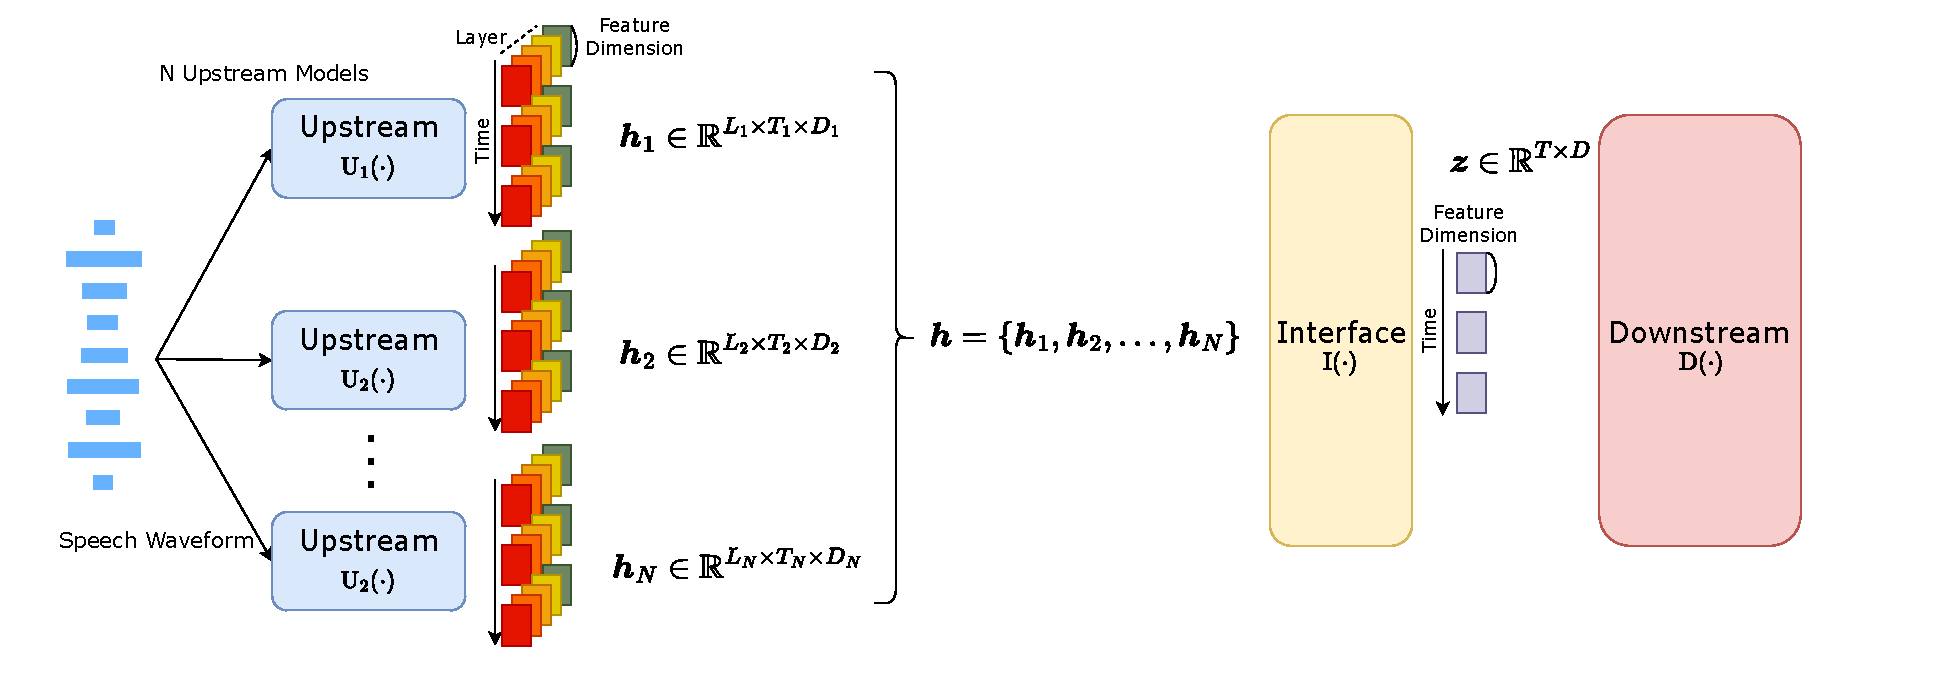
\includegraphics[width=\linewidth,trim={0.8cm 0.3cm 2.2cm 0.2cm},clip]{figs/FusionInterface-FusionOverview_long2.pdf}
   \vspace{-20pt}
  \caption{An overview framework of Interface with fusion.}
  \label{fig:overview}
\vspace{-15pt}
\end{figure*}

% Argue that model fusion and layer selection is the same concept
In this work, we argue for a unified framework that jointly considers model fusion and layer fusion. 
To the best of our knowledge,~\cite{chiu24_sinica} is the first attempt to jointly address model fusion and layer selection, but their approach still treats the two processes separately by independently performing layer fusion within each model before applying model fusion. 
Moreover, \cite{chiu24_sinica} finds that there is no single combination of model and layer fusion that consistently performs well regardless of the chosen upstream model.
Also, their evaluation is limited only to the ASR task on LibriSpeech using self-supervised foundation models.

Our work addresses these limitations in several ways. 
First, we unify model fusion and layer fusion into a single module and demonstrate that optimizing them jointly significantly outperforms the method proposed by \cite{chiu24_sinica}. 
Second, our evaluation spans multiple ASR and non-ASR tasks, including Emotion Recognition and Speaker Verification, and we show consistent improvements across these tasks using our proposed method. 
Finally, we consider the fusion of both supervised and self-supervised speech models and find that their fusion outperforms that of fusing solely self-supervised models.



% Motivated by these limitations, we first extend the interface proposed by ~\cite{shih24_interface} to incorporate model fusion.
% We also propose a revised version of the Hierarchical Convolution interface that enables simultaneous fusion of multiple upstream models and their layers.
% Our evaluation spans multiple ASR and non-ASR tasks, including Emotion Recognition and Speaker Verification. 
% Furthermore, we compare the fusion of both supervised and self-supervised speech models.



% Our results indicate that our revised Hierarchical Interface consistently outperforms prior approaches for the majority of tasks and models. 
% We also emphasize the importance of selecting suitable upstream model combinations, as the choice of models significantly impacts overall performance. 
In conclusion, our contributions can be summarized as follows:
\begin{enumerate}
    \item We introduce a novel technique for unifying and jointly optimizing model and layer fusion, and show that it outperforms prior work which optimizes these separately.
    \item Our work is the first to conduct thorough experiments on SFM fusion across both ASR and non-ASR tasks.
    \item In most cases, our proposed fusion method outperforms prior methods for various upstream models. We also observe the best performance when fusing self-supervised with traditional supervised speech models, indicating that these models learn to model different and complementary aspects of the speech signal.
\end{enumerate}

% ~\\
% ~\\
% ~\\
% ~\\
% ~\\
% ~\\
% ~\\
% ~\\
% ~\\
% ~\\
% ~\\
% ~\\
% ~\\
% ~\\
% ~\\
% ~\\
% ~\\
% ~\\
% ~\\
% ~\\
% ~\\
% ~\\
% ~\\
% ~\\
% ~\\
% ~\\
% ~\\
% ~\\
% ~\\
